
Epitaxial layer thickness: più grande è e più carica viene depositata da una MIP, però devi fare attenzione alla forma della zona svuotata perchè può portare ad un aumento della charge sharing tra pixel vicini. Se il diodo è molto piccolo rischi che l'efficienza di collection è diminutia perchè l'intensità del campo elettrico è più bassa intorno al diodo, e hai più charge sharing.\\
50x50 um2 e l'elettrodo è 3 um

\begin{figure}[h!]
    \centering
    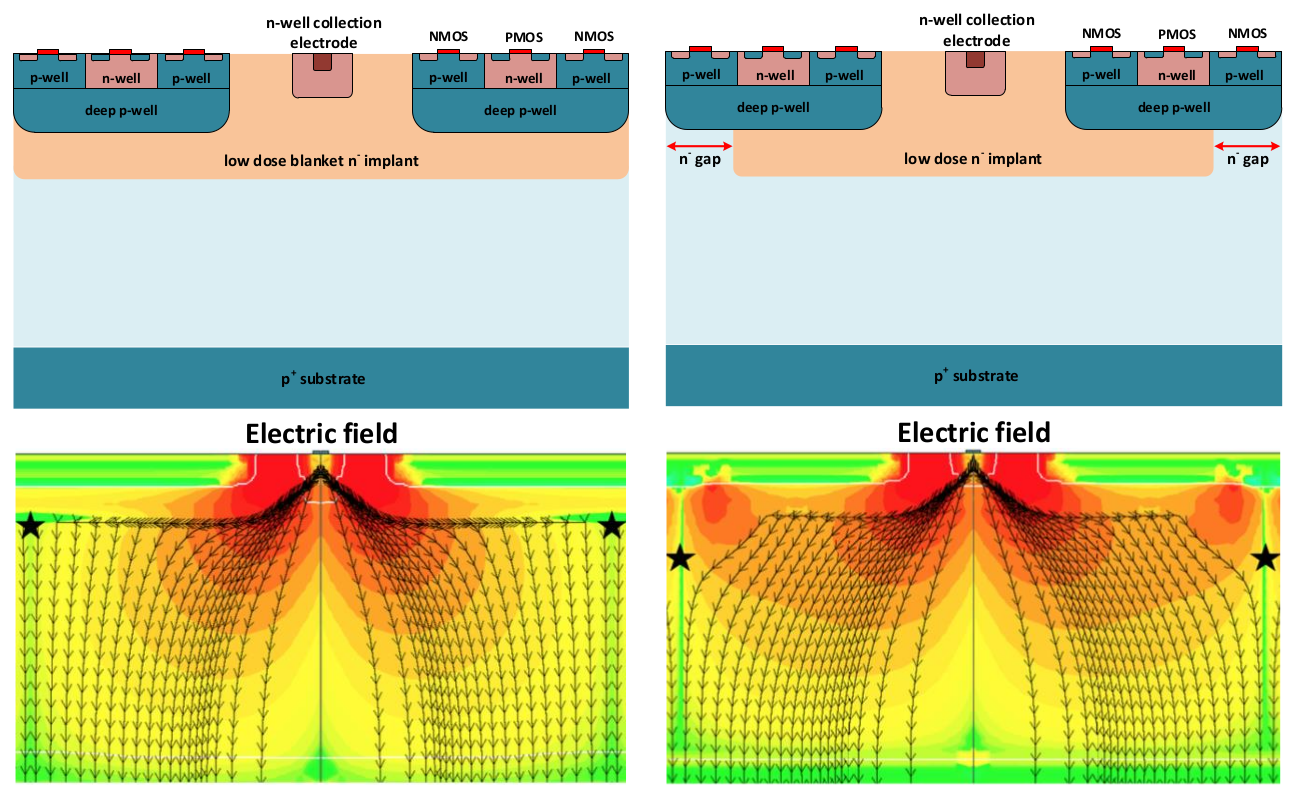
\includegraphics[width=.9\linewidth]{figures/Monopix1/Monopix1_section_scheme.png}
    \caption{Cross scheme of a modified sensor of TJ-Monopix1}
    \label{fig:Monopix1_section_scheme}
 \end{figure}


\section{FE flavors}
    INput coupling: differenza tra AC (flavor HV) e DC. 4 flavors\\
    \begin{figure}[h!]
        \centering
        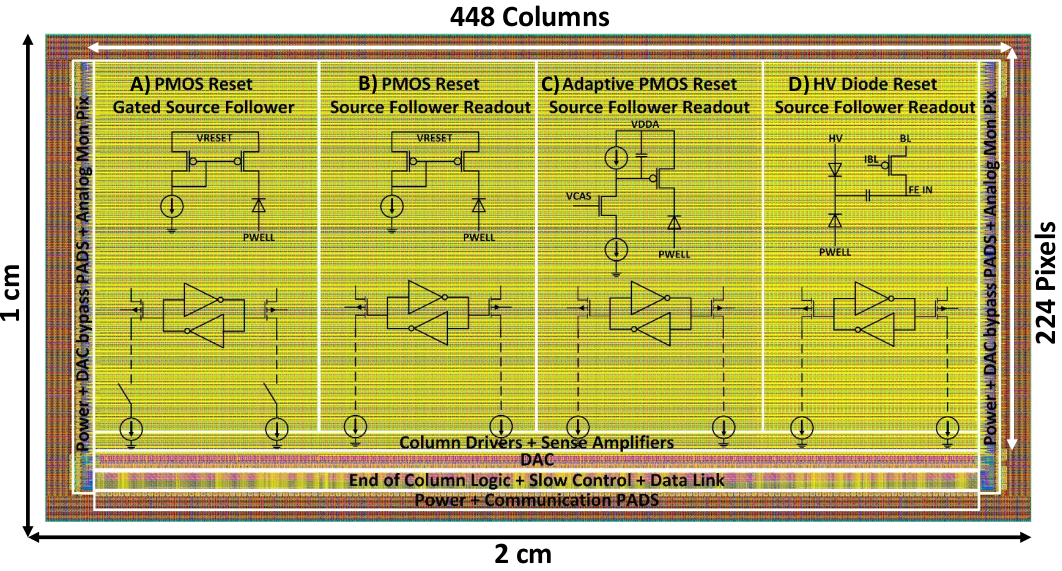
\includegraphics[width=.7\linewidth]{figures/Monopix1/Monopix1_flavors.png}
        \caption{}
        \label{fig:Monopix1_flavors}
    \end{figure}


    \begin{figure}[h!]
        \centering
        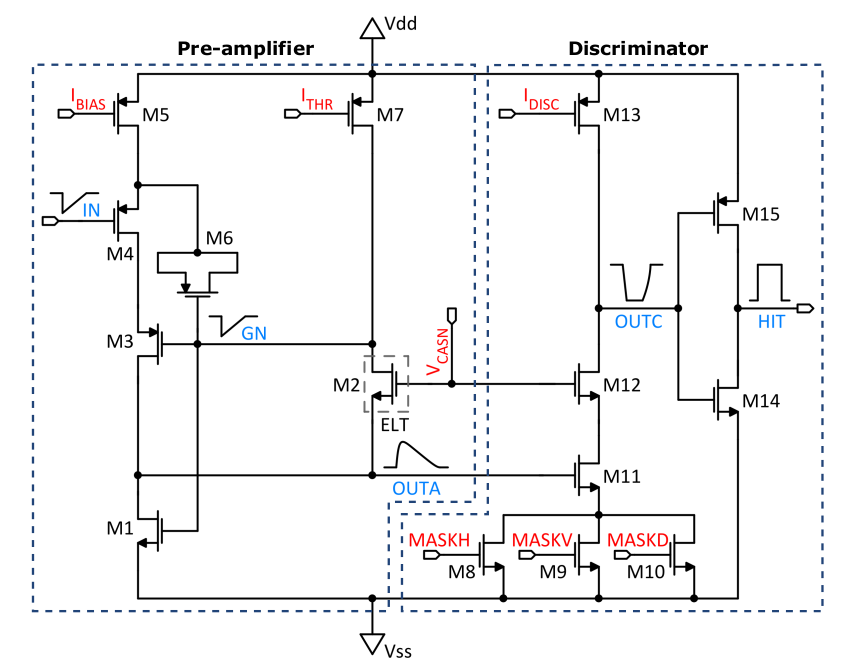
\includegraphics[width=.7\linewidth]{figures/Monopix1/Monopix1_FE_circuit.png}
        \caption{}
        \label{fig:Monopix1_FE_circuit}
    \end{figure}

        R resistenza di reset deve essere abbastanza grande in modo da far si che il
    ritorno allo zero è abbastanza lento (non devi "interferire" con la tot slope
    e non devi più corto del tempo del preamplificatore, sennò hai perdita di segnale).\\
    Baseline reset: all'input solitamente hai un PMOSS o un diodo;  
    Voltage amplifier: perchè? ripeti un attimo il vantaggio. \\
    Source follower per disaccoppiare shaper e LF feedback.\\


\section{Readout logic}
    viene da lf monopix\\
    TJ monopix ha un colum drain readout proven by the ATLAS FEI3 front end chip (
    I. Peric et al., The FEI3 readout chip for the ATLAS pixel detector,
    Nucl. Instrum. Meth. A 565 (2006) 178, ed. by J. Grosse-Knetter, H. Krueger, and N. Wermes
    (cit. on pp. 42, 50, 60))\\

    TJ-Monopix is a triggerless. It sends data whenever it gets hits. Only thing we can do is to record timetamp of the external triggers and correlate with the hits. 
    \begin{figure}[h!]
        \centering
        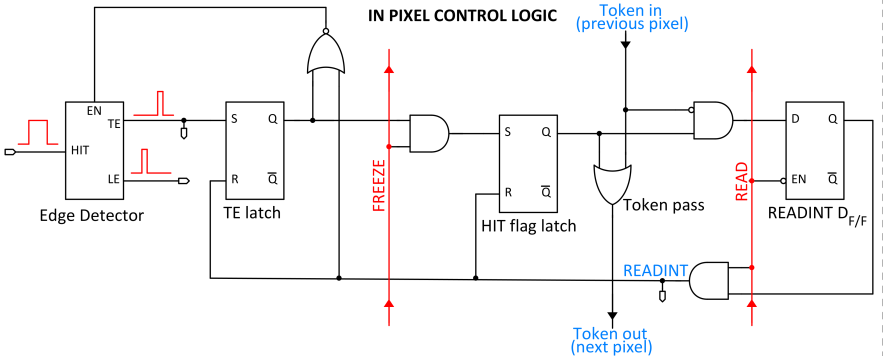
\includegraphics[width=.7\linewidth]{figures/Monopix1/Monopix1_readout_schematics.png}
        \caption{}
        \label{fig:Monopix1_readout_schematics}
    \end{figure}

    \begin{figure}[h!]
        \centering
        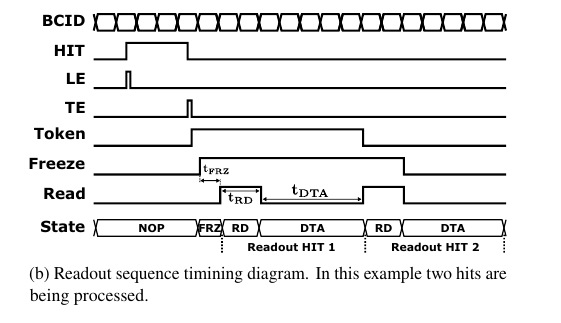
\includegraphics[width=.7\linewidth]{figures/Monopix1/readout_timing.png}
        \caption{}
        \label{fig:readout_timing}
    \end{figure}
    

    \subsection{Data-packets structure}

    \subsection{Dead time measurement}

\section{From TJ-Monopix1 to Obelix}
    Subm. Aug. 2016, mentre monopix 2 sub a aprile 2020\\

    \begin{figure}[h!]
        \centering
        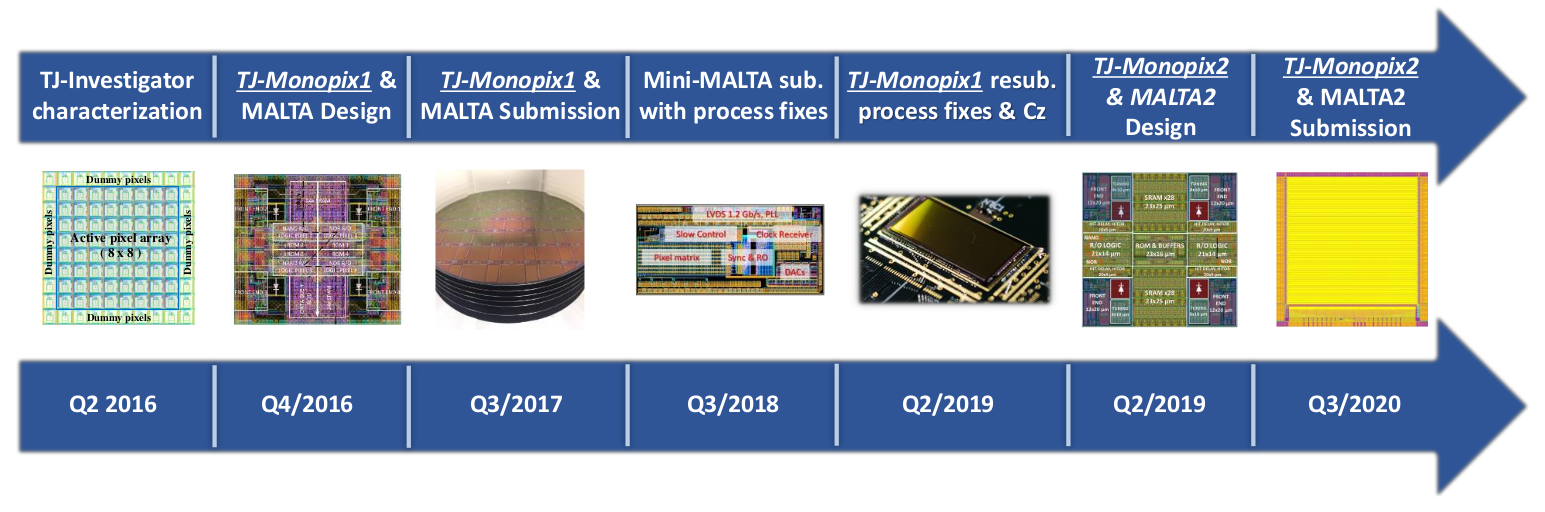
\includegraphics[width=.7\linewidth]{figures/Monopix1/TJ180nm.png}
        \caption{}
        \label{fig:TJ180nm}
    \end{figure}

